\section{Week 4}
\textbf{$\mathcal{Z}$-transform}

\begin{equation*}
    z = e^{sT}
\end{equation*}
\begin{align*}
        y(k+1) + y(k) - y(k-1) &= u(k) \\
        \xrightarrow{\mathcal{Z}} zY(z) + Y(z) - z^{-1} Y(z) &= U(z)
\end{align*}

\textbf{Transfer function of ZOH}
\begin{equation*}
    G_{ZOH}(s) = \frac{1-e^{-sT}}{s} 
\end{equation*}

\textbf{Transfer function of ZOH and Analogy System (ZAS)}
\begin{align*}
    G_{ZAS}(z) &= \mathcal{Z}\left\{\frac{1-e^{-sT}}{s}G_{p}(s)\right\} \\
    &=  (1-z^{-1})\mathcal{Z}\left\{\frac{G_p (s)}{s}\right\} \\
    &= \frac{z-1}{z} \mathcal{Z}\left\{\frac{G_p (s)}{s}\right\}
\end{align*}

\textbf{Trick for finding inverse $\mathcal{Z}$-transform}

Divide the expression by z first, then find inverse using tables.

Example:
\begin{align*}
    Y(z) &= \frac{z^2}{(z-1)(z-0.5) } \\
    \frac{Y(z)}{z} &= \frac{z}{(z-1)(z-0.5)} = \frac{2}{z-1} - \frac{1}{z-0.5} \\
    Y(z) &= \frac{2z}{z-1} - \frac{z}{z-0.5} \\
    y(k) &= \mathcal{Z}^{-1}\left\{\frac{2z}{z-1}\right\} - \mathcal{Z}^{-1}\left\{ \frac{z}{z-0.5}\right\} \\
    &= 2 - 0.5^{k}
\end{align*}

\textbf{Associativity of Continuous Transfer Functions}
\begin{figure}[H]
    \centering
    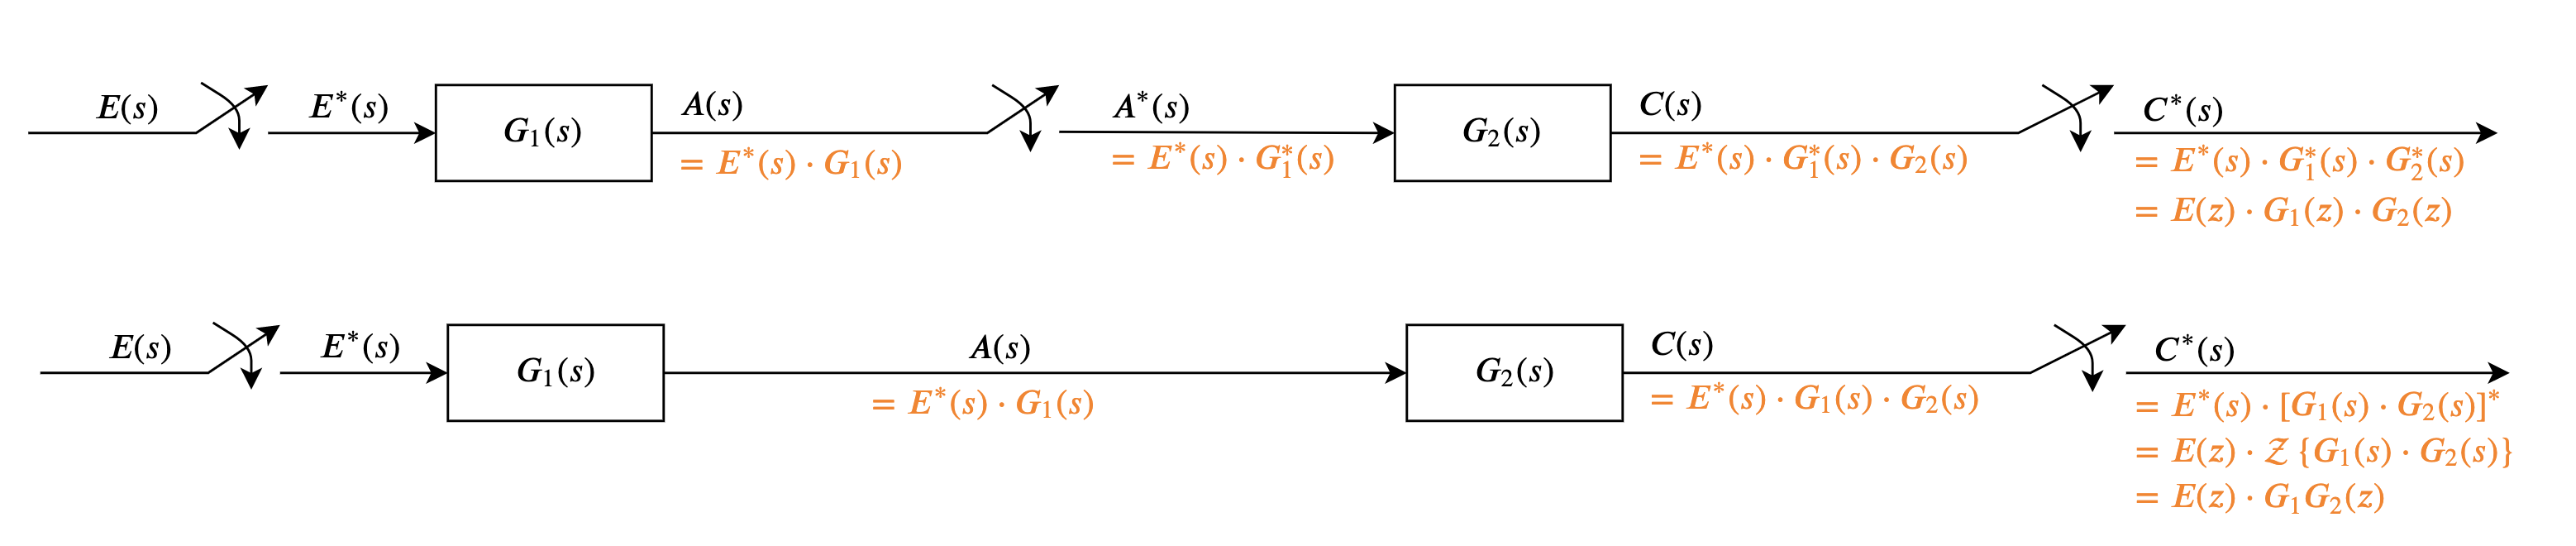
\includegraphics[width=0.5\textwidth]{images/associativity.png}
\end{figure}
Be careful: only distribute the * sign among addition/subtraction!